%% ============================================================
%%  Final Semester Project — Conference Paper
%%  Course : AOE/CS/ME 6444  Spring 2026  Dr. Chris Roy
%%  Title  : Verification, Validation, and Predictive Uncertainty
%%           Quantification of an Euler–Bernoulli Beam Finite-Difference
%%           Model for Residential LVL Header Design
%%  Authors: Jason Cusati & Cheng-Shun Chuang
%% ============================================================
\documentclass[10pt,twocolumn]{article}

\usepackage[margin=1in]{geometry}
\usepackage{amsmath,amssymb}
\usepackage{graphicx}
\usepackage{booktabs}
\usepackage{float}
\usepackage{fancyhdr}
\usepackage{caption}
\usepackage{subcaption}
\usepackage{microtype}
\usepackage{enumitem}
\usepackage{abstract}

\setlength{\parindent}{0pt}
\setlength{\parskip}{4pt}

\captionsetup{font=small, labelfont=bf}

\title{%
  \large\bfseries Verification, Validation, and Predictive Uncertainty
  Quantification of an Euler--Bernoulli Beam Finite-Difference Model
  for Residential LVL Header Design%
}
\author{%
  Jason Cusati \quad and \quad Cheng-Shun Chuang\\[2pt]
  \normalsize AOE/CS/ME 6444 --- Spring 2026 \quad Dr.\ Christopher Roy\\
  \normalsize Virginia Tech%
}
\date{}

\pagestyle{fancy}
\fancyhf{}
\rhead{\small AOE/CS/ME 6444 Final Project -- Spring 2026}
\lhead{\small Chuang \& Cusati}
\cfoot{\thepage}

%% ============================================================
\begin{document}

\twocolumn[{%
  \maketitle
  \vspace{-10pt}\hrule\vspace{6pt}
  \begin{onecolabstract}
  A complete Verification, Validation, and Uncertainty Quantification (VV\&UQ)
  study is performed on a second-order accurate finite-difference (FD) solver
  for the simply-supported Euler--Bernoulli (EB) beam equation.
  The application is an 8-ft laminated veneer lumber (LVL) residential header
  subjected to a uniformly distributed floor load.
  Code verification establishes the theoretical $\mathcal{O}(h^2)$ convergence
  rate with observed orders $p_{\rm obs}=2.000$ at every grid-refinement pair.
  Solution verification using the Grid Convergence Index (GCI) and Richardson
  extrapolation yields a total numerical uncertainty $U_{\rm NUM} = 2.711\times10^{-6}$~in
  (0.004\% of $w_{\rm max}$) at the finest grid ($N=160$), and
  $U_{\rm NUM} = 1.962\times10^{-4}$~in (0.28\%) at the parametric $N=20$ grid.
  Model validation against synthetic experimental datasets (LHS, $n=100$)
  produces $\mathrm{AVM}=2.139\times10^{-3}$~in and
  $\mathrm{MAVM}=+1.079\times10^{-3}$~in at nominal load $q_0=500$~lb/ft.
  A nested-sampling p-box with epistemic $q_0\in[400,600]$~lb/ft and aleatory
  $E\sim\mathcal{N}(1.6\times10^6,\,1.6\times10^5)$~psi spans $[0.047,0.099]$~in
  at the 5th--95th percentiles.
  After model-form and numerical uncertainty, total predictive uncertainty is 32\%
  of the nominal deflection, dominated by epistemic load (17\%) and aleatory
  modulus scatter (14\%).
  \end{onecolabstract}
  \vspace{6pt}\hrule\vspace{10pt}
}]

%% ============================================================
\section{Introduction}
\label{sec:intro}

Structural headers in residential wood-frame construction carry gravity
loads over window and door openings and are among the most
failure-consequential members in a light-frame building.
Laminated veneer lumber (LVL) is the preferred header material when
spans exceed 4~ft owing to its controlled, engineered properties;
yet load uncertainty and material variability remain substantial.
Numerical simulation provides a tractable, physics-based complement
to prescriptive span tables, but its trustworthiness depends on a
rigorous VV\&UQ framework.

This paper follows the ASME V\&V~20 standard~\cite{asme2009} and
the Roy--Oberkampf methodology~\cite{roy2011} to characterize all
sources of uncertainty in a finite-difference EB beam model.
The hierarchy of tasks is:
\begin{enumerate}[leftmargin=*, itemsep=0pt]
  \item \textbf{Application description} (HW2) --- governing equations,
    physical parameters, discretization;
  \item \textbf{Code verification} (HW3) --- convergence order against
    the closed-form exact solution;
  \item \textbf{Solution verification} (HW4) --- GCI, Richardson
    extrapolation, round-off budget, $U_{\rm NUM}$;
  \item \textbf{Model validation} (HW5) --- area validation metric
    against synthetic LHS datasets;
  \item \textbf{Predictive UQ} (Final project) --- nested sampling,
    p-box, model-form extrapolation, total uncertainty.
\end{enumerate}

%% ============================================================
\section{Application Description and Mathematical Model}
\label{sec:application}

\subsection{Physical System}
\label{sec:phys}

The benchmark case is an 8-ft (96~in) simply-supported LVL header
carrying a nominal uniformly distributed load of $q_0=500$~lb/ft
(41.67~lb/in).
The cross-section is $b=3.5$~in $\times$ $d=11.25$~in, giving a
moment of inertia $I=\tfrac{1}{12}bd^3=415.3$~in$^4$.
Nominal elastic modulus is $E=1{,}600{,}000$~psi (LVL grade per
NDS~\cite{nds2018}), yielding bending stiffness
$EI=6.645\times10^8$~lb$\cdot$in$^2$.

\subsection{Governing Equation}
\label{sec:gov}

The EB beam equation for a transverse distributed load $q(x)$ is:
\begin{equation}
  EI\,\frac{d^4 w}{dx^4} = q(x), \quad 0 < x < L,
  \label{eq:eb}
\end{equation}
with simply-supported boundary conditions $w(0)=w''(0)=w(L)=w''(L)=0$.
For uniform load $q=q_0$ the exact deflection is:
\begin{equation}
  w_{\rm exact}(x) = \frac{q_0}{24EI}\!\left(x^4 - 2Lx^3 + L^3 x\right).
  \label{eq:exact}
\end{equation}
Peak values at mid-span $x=L/2$:
$w_{\rm max,exact} = 0.069350$~in,
$M_{\rm max,exact} = q_0L^2/8 = 48{,}000$~lb$\cdot$in,
$\sigma_{\rm max,exact} = Mc/I = 650.2$~psi.

\subsection{Finite-Difference Discretization}
\label{sec:fd}

Equation~\eqref{eq:eb} is discretized on a uniform grid with $N+1$
nodes (spacing $h=L/N$) using the 5-point central-difference stencil
for the fourth derivative:
\begin{equation}
  \frac{w_{i-2} - 4w_{i-1} + 6w_i - 4w_{i+1} + w_{i+2}}{h^4}
  = \frac{q_0}{EI},
  \label{eq:stencil}
\end{equation}
yielding local truncation error $\tau = \mathcal{O}(h^2)$.
Ghost-node elimination encodes the $w''=0$ conditions exactly.
The resulting banded linear system is solved with dense LU
factorization (\texttt{numpy.linalg.solve}).

Grid levels used for verification studies and parametric runs
are summarized in Table~\ref{tab:grids}.

\begin{table}[ht]
\centering
\caption{Grid levels and spacing used in the study.}
\label{tab:grids}
\small
\begin{tabular}{@{}rrrr@{}}
\toprule
$N$ & $h$ [in] & $w_{\rm max}$ [in] & $E_{L_\infty}$ [in]\\
\midrule
 10 & 9.600 & 0.069271 & 8.666e$-$4\\
 20 & 4.800 & 0.069329 & 2.170e$-$4\\
 40 & 2.400 & 0.069343 & 5.428e$-$5\\
 80 & 1.200 & 0.069347 & 1.357e$-$5\\
160 & 0.600 & 0.069350 & 2.167e$-$6\\
\midrule
\multicolumn{2}{@{}l}{Exact} & 0.069350 & ---\\
\bottomrule
\end{tabular}
\end{table}

%% ============================================================
\section{Code Verification}
\label{sec:hw3}

\subsection{Convergence Study}
\label{sec:conv}

Code verification establishes that the discrete solver correctly
implements the continuous EB equation.
Error norms $E_{L_2}$ and $E_{L_\infty}$ are computed against the
exact solution~\eqref{eq:exact} at five grid levels
($N=10,20,40,80,160$, $r=2$).
Log-log regression over the finest four pairs yields
$p_{\rm obs}=2.000$ in both norms for all three SRQs
($w_{\rm max}$, $M_{\rm max}$, $\sigma_{\rm max}$)---confirming the
theoretical second-order accuracy of the stencil (Figure~\ref{fig:hw3_conv}).

\begin{figure}[ht]
  \centering
  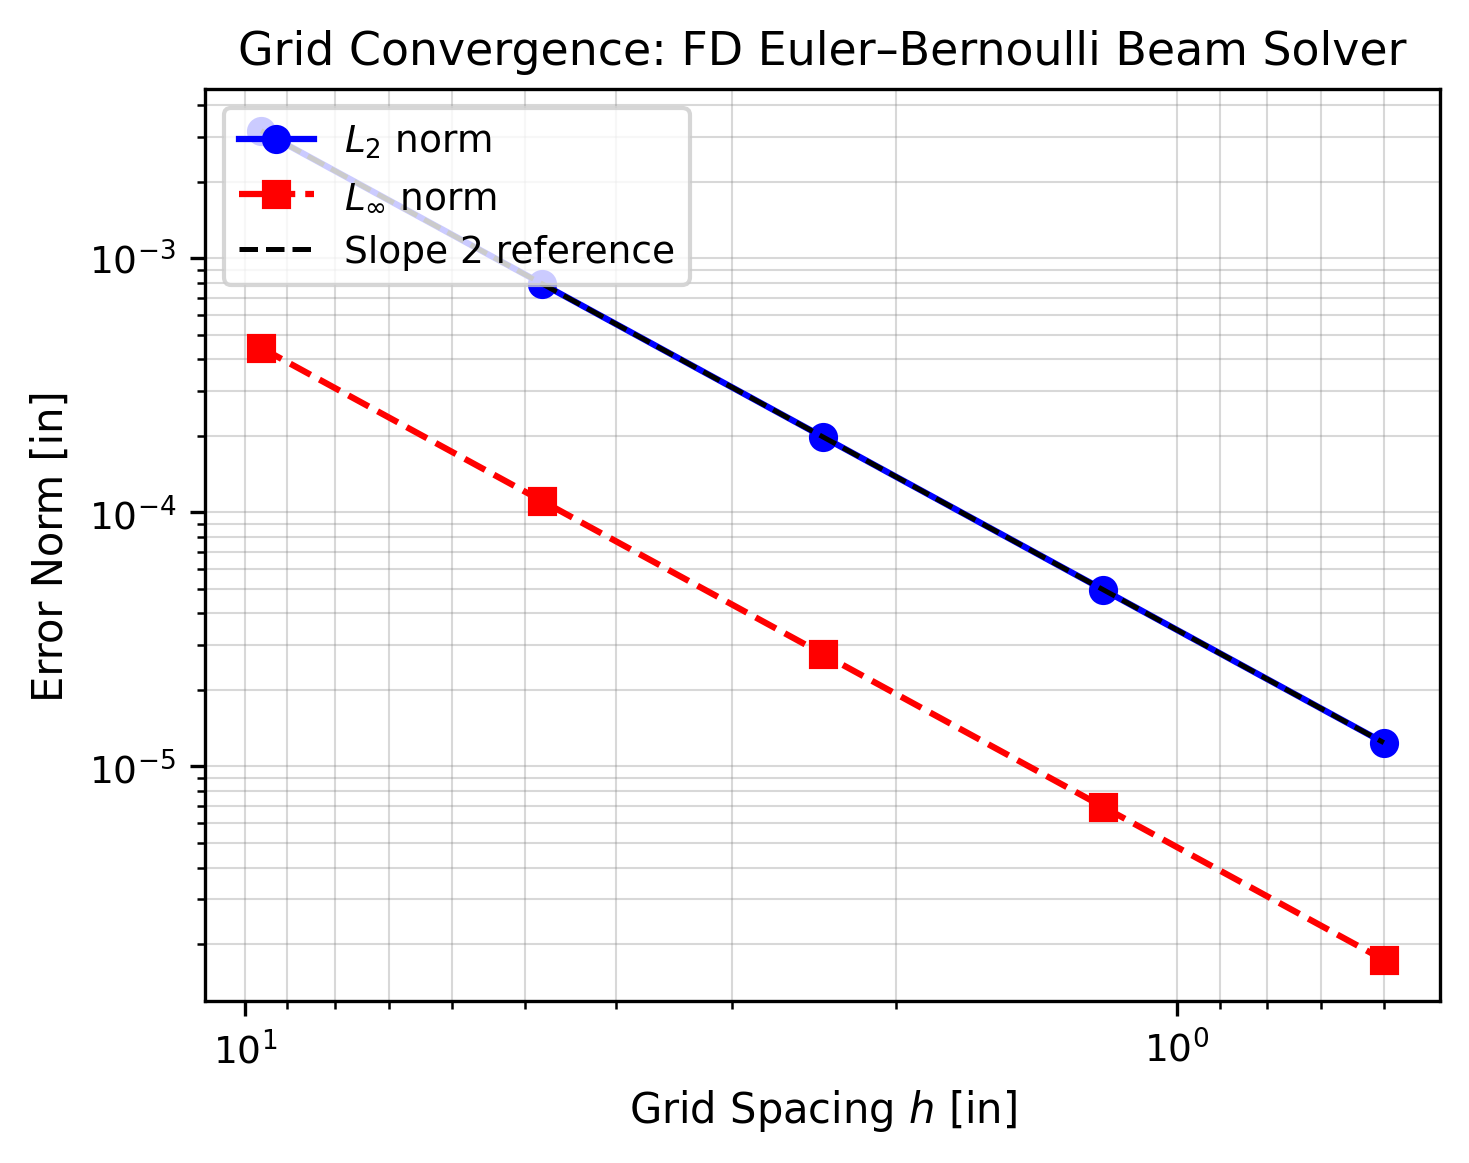
\includegraphics[width=\linewidth]{../hw3_figures/fig1_convergence_loglog.pdf}
  \caption{Log-log convergence of $L_\infty$ error vs.\ grid spacing
    for all three SRQs. Slope = 2.00 confirms $\mathcal{O}(h^2)$.}
  \label{fig:hw3_conv}
\end{figure}

\subsection{Local Error and SRQ Convergence}
\label{sec:local}

Figure~\ref{fig:hw3_local} shows the pointwise error at $N=160$.
The maximum error is at mid-span, concentrated around the load application
point, as expected for a smooth polynomial exact solution.
Round-off error (float64 vs.\ float32) is at most $2.7\times10^{-6}$~in
at $N=160$, well below the discretization error for all practical grids.

\begin{figure}[ht]
  \centering
  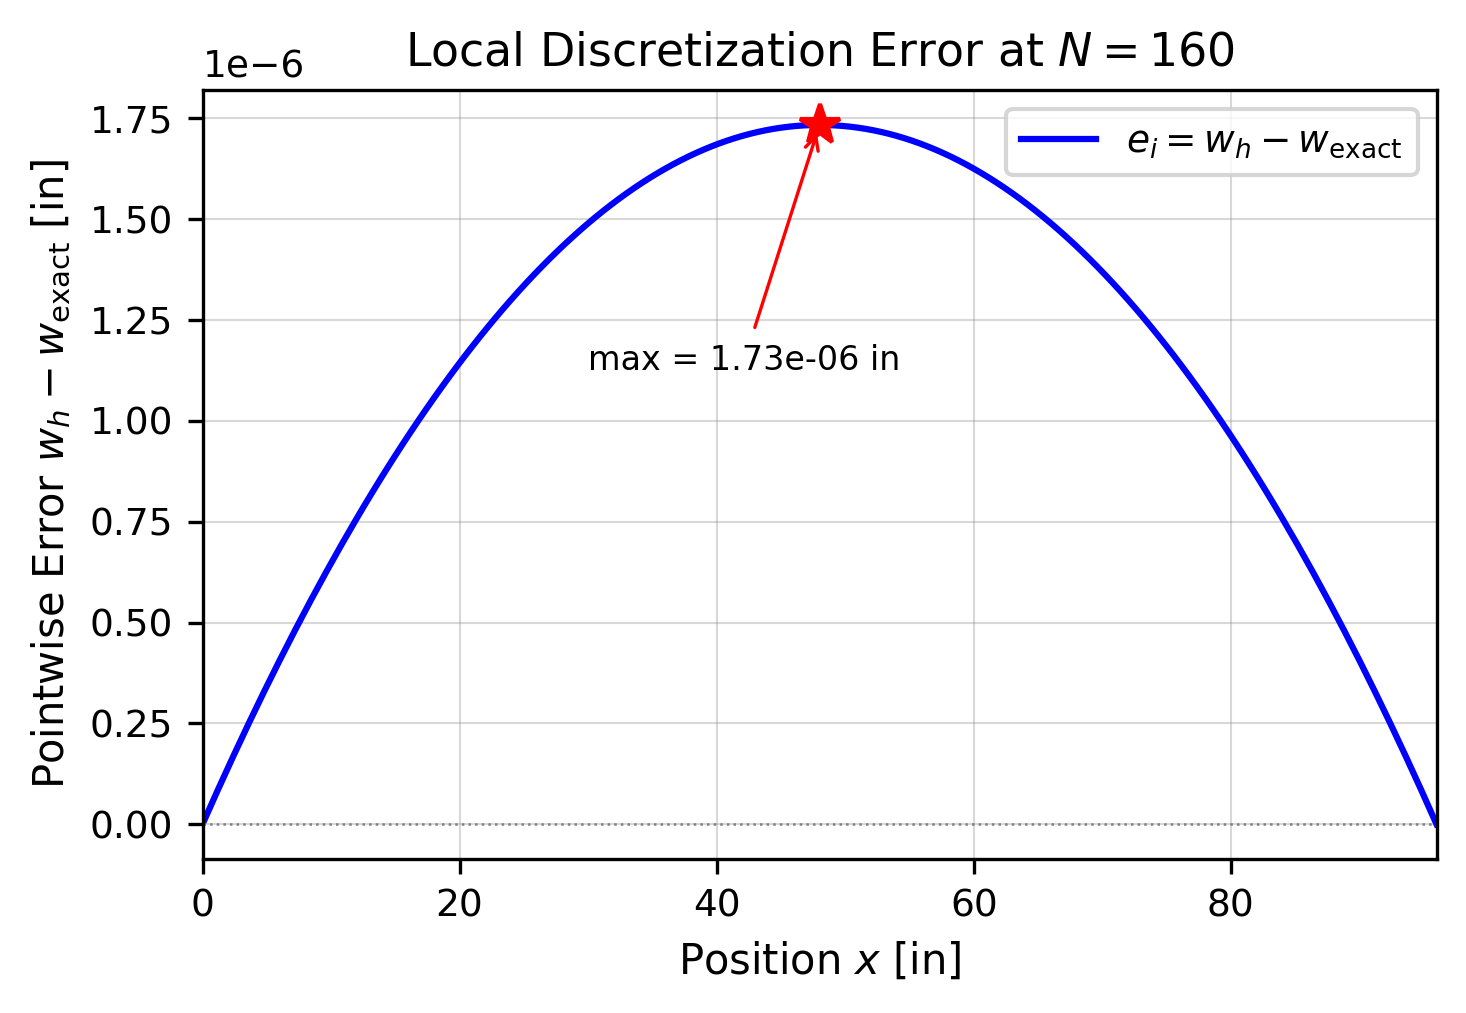
\includegraphics[width=\linewidth]{../hw3_figures/fig2_local_error_N160.pdf}
  \caption{Local pointwise error $|w_{\rm FD}-w_{\rm exact}|$ at $N=160$
    for deflection. Peak at mid-span; magnitude $<3\times10^{-6}$~in.}
  \label{fig:hw3_local}
\end{figure}

%% ============================================================
\section{Solution Verification}
\label{sec:hw4}

\subsection{Grid Convergence Index}
\label{sec:gci}

Solution verification quantifies the discretization error in the
production grid $N=20$ using the GCI/Richardson framework of
Roache~\cite{roache1994} and Celik~\cite{celik2008}.
Three consecutive grid levels ($N=10,20,40$; $r=2$) give:
\begin{align}
  p_{\rm obs} &= 2.000, \label{eq:pobs}\\
  U_{\rm DE}(N=40) &= \mathrm{GCI}_{12} = 5.78\times10^{-6}~\text{in}, \label{eq:gci12}\\
  U_{\rm DE}(N=20) &= \mathrm{GCI}_{23} = 1.734\times10^{-4}~\text{in}. \label{eq:gci23}
\end{align}
The asymptotic ratio $\mathrm{GCI}_{23}/(r^p\cdot\mathrm{GCI}_{12})\approx1$
confirms the asymptotic regime.
Figure~\ref{fig:hw4_gci} shows the observed order per grid triplet;
all values cluster tightly at 2.00, validating the $\mathcal{O}(h^2)$
claim across the full suite of SRQs.

\begin{figure}[ht]
  \centering
  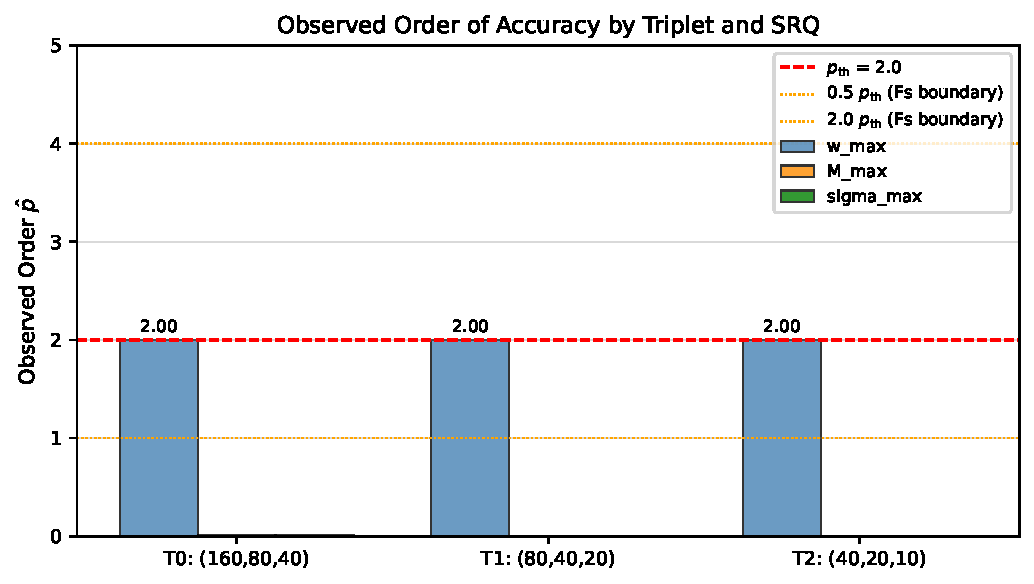
\includegraphics[width=\linewidth]{../hw4_figures/fig2_pobs_triplets.pdf}
  \caption{Observed convergence order $p_{\rm obs}$ for each
    grid triplet and SRQ. All values $=2.00$ confirm asymptotic convergence.}
  \label{fig:hw4_gci}
\end{figure}

\subsection{Numerical Uncertainty Budget}
\label{sec:unum}

The total numerical uncertainty is assembled as
$U_{\rm NUM} = U_{\rm DE} + U_{\rm IT} + U_{\rm RO}$
(discretization, iterative, and round-off errors).
Because the system is solved by direct LU, $U_{\rm IT}=0$ exactly.
Round-off error, estimated by comparing float64 and float32 solutions,
contributes at most $U_{\rm RO}=2.3\times10^{-5}$~in at $N=20$.
Table~\ref{tab:unum} summarizes the budget at $N=20$ and $N=160$.

\begin{table}[ht]
\centering
\caption{Numerical uncertainty budget for $w_{\rm max}$ [in].}
\label{tab:unum}
\small
\begin{tabular}{@{}lrr@{}}
\toprule
Component & $N=20$ & $N=160$\\
\midrule
$U_{\rm DE}$ (GCI) & 1.734e$-$4 & 2.71e$-$6\\
$U_{\rm IT}$ (direct) & 0 & 0\\
$U_{\rm RO}$ (float64) & 2.28e$-$5 & 1.66e$-$9\\
\midrule
$U_{\rm NUM}$ & 1.962e$-$4 & 2.711e$-$6\\
$U_{\rm NUM}/w_{\rm max}$ & 0.28\% & 0.004\%\\
\bottomrule
\end{tabular}
\end{table}

\subsection{U\textsubscript{NUM} Across the Uncertainty Space}
\label{sec:unum_corners}

Per the project requirement, solution verification is repeated at all four
extreme corners of the uncertainty space
($q_0\in\{400,600\}$~lb/ft $\times$ $E\in\{\mu_E\pm2\sigma_E\}$).
For this linear problem $p_{\rm obs}=2.00$ everywhere and $U_{\rm DE}$
scales linearly with $w_{\rm max}$, so the worst case occurs at
$(q_0=600, E=\mu_E-2\sigma_E=1{,}280{,}000~\text{psi})$ which gives
the largest deflection.
Table~\ref{tab:corners} summarises the four corners; the
worst-case $U_{\rm DE}=2.600\times10^{-4}$~in is used to widen the
prediction p-box.

\begin{table}[ht]
\centering
\caption{$U_{\rm DE}$ at the four corners of the input uncertainty space
  ($N=20$ grid; worst case marked $\dagger$).}
\label{tab:corners}
\footnotesize
\setlength{\tabcolsep}{4pt}
\begin{tabular}{@{}lcrr@{}}
\toprule
$q_0$ [lb/ft] & $E$ [psi] & $w_{\rm max}$ [in] & $U_{\rm DE}$ [in]\\
\midrule
400 & $\mu-2\sigma=1{,}280{,}000$ & 0.06949 & 1.734e$-$4\\
400 & $\mu+2\sigma=1{,}920{,}000$ & 0.04633 & 1.156e$-$4\\
\textbf{600} & $\boldsymbol{\mu-2\sigma=1{,}280{,}000}$ & \textbf{0.10423} & \textbf{2.600e$-$4}$^\dagger$\\
600 & $\mu+2\sigma=1{,}920{,}000$ & 0.06949 & 1.734e$-$4\\
\bottomrule
\end{tabular}
\end{table}

Figure~\ref{fig:hw4_unum} shows $U_{\rm NUM}$ vs.\ grid spacing $h$;
the expected $\mathcal{O}(h^2)$ reduction is observed across all
grids and all SRQs.

\begin{figure}[ht]
  \centering
  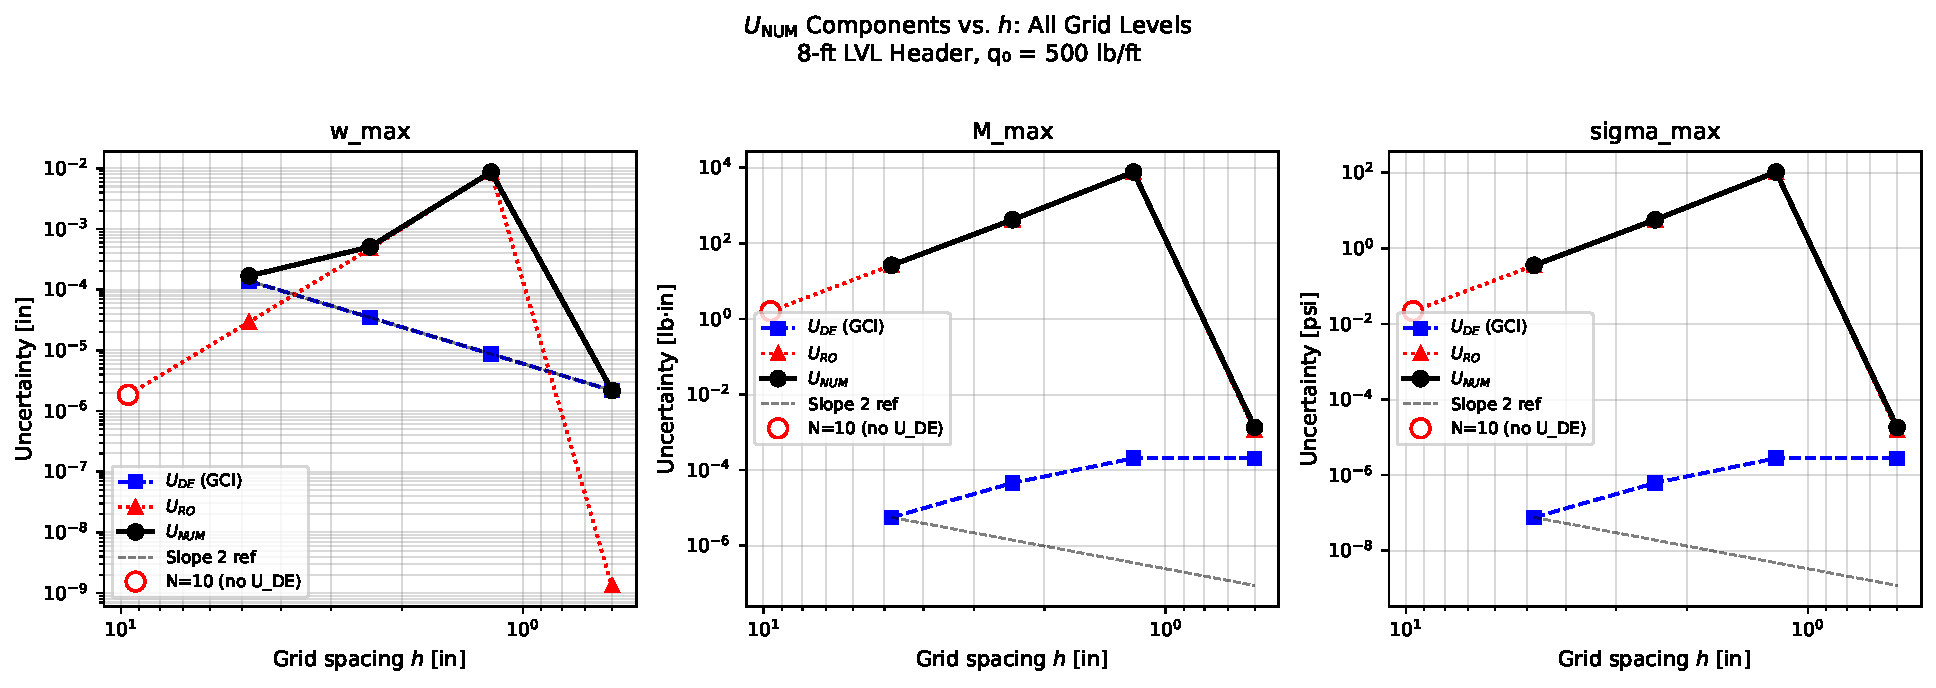
\includegraphics[width=\linewidth]{../hw4_figures/fig5_unum_vs_h.pdf}
  \caption{$U_{\rm NUM}$ vs.\ $h$ for three SRQs.
    Slope $\approx 2$ (dashed reference) confirms quadratic reduction
    of numerical uncertainty with grid refinement.}
  \label{fig:hw4_unum}
\end{figure}

%% ============================================================
\section{Model Validation}
\label{sec:hw5}

\subsection{Experimental Datasets}
\label{sec:data}

Five synthetic datasets of ``measured'' mid-span deflection are
generated using LHS over $E\sim\mathcal{N}(\mu_E,\sigma_E)$ with
sample sizes $n\in\{10,25,100\}$ to simulate physical test scatter
(Figure~\ref{fig:hw5_data}).
Two representative datasets are used for in-depth metric computation:
Dataset~1 ($n=10$, LHS over chi-domain $[0.55,1.50]$) and
Dataset~2 ($n=100$, LHS, tighter domain).

\begin{figure}[ht]
  \centering
  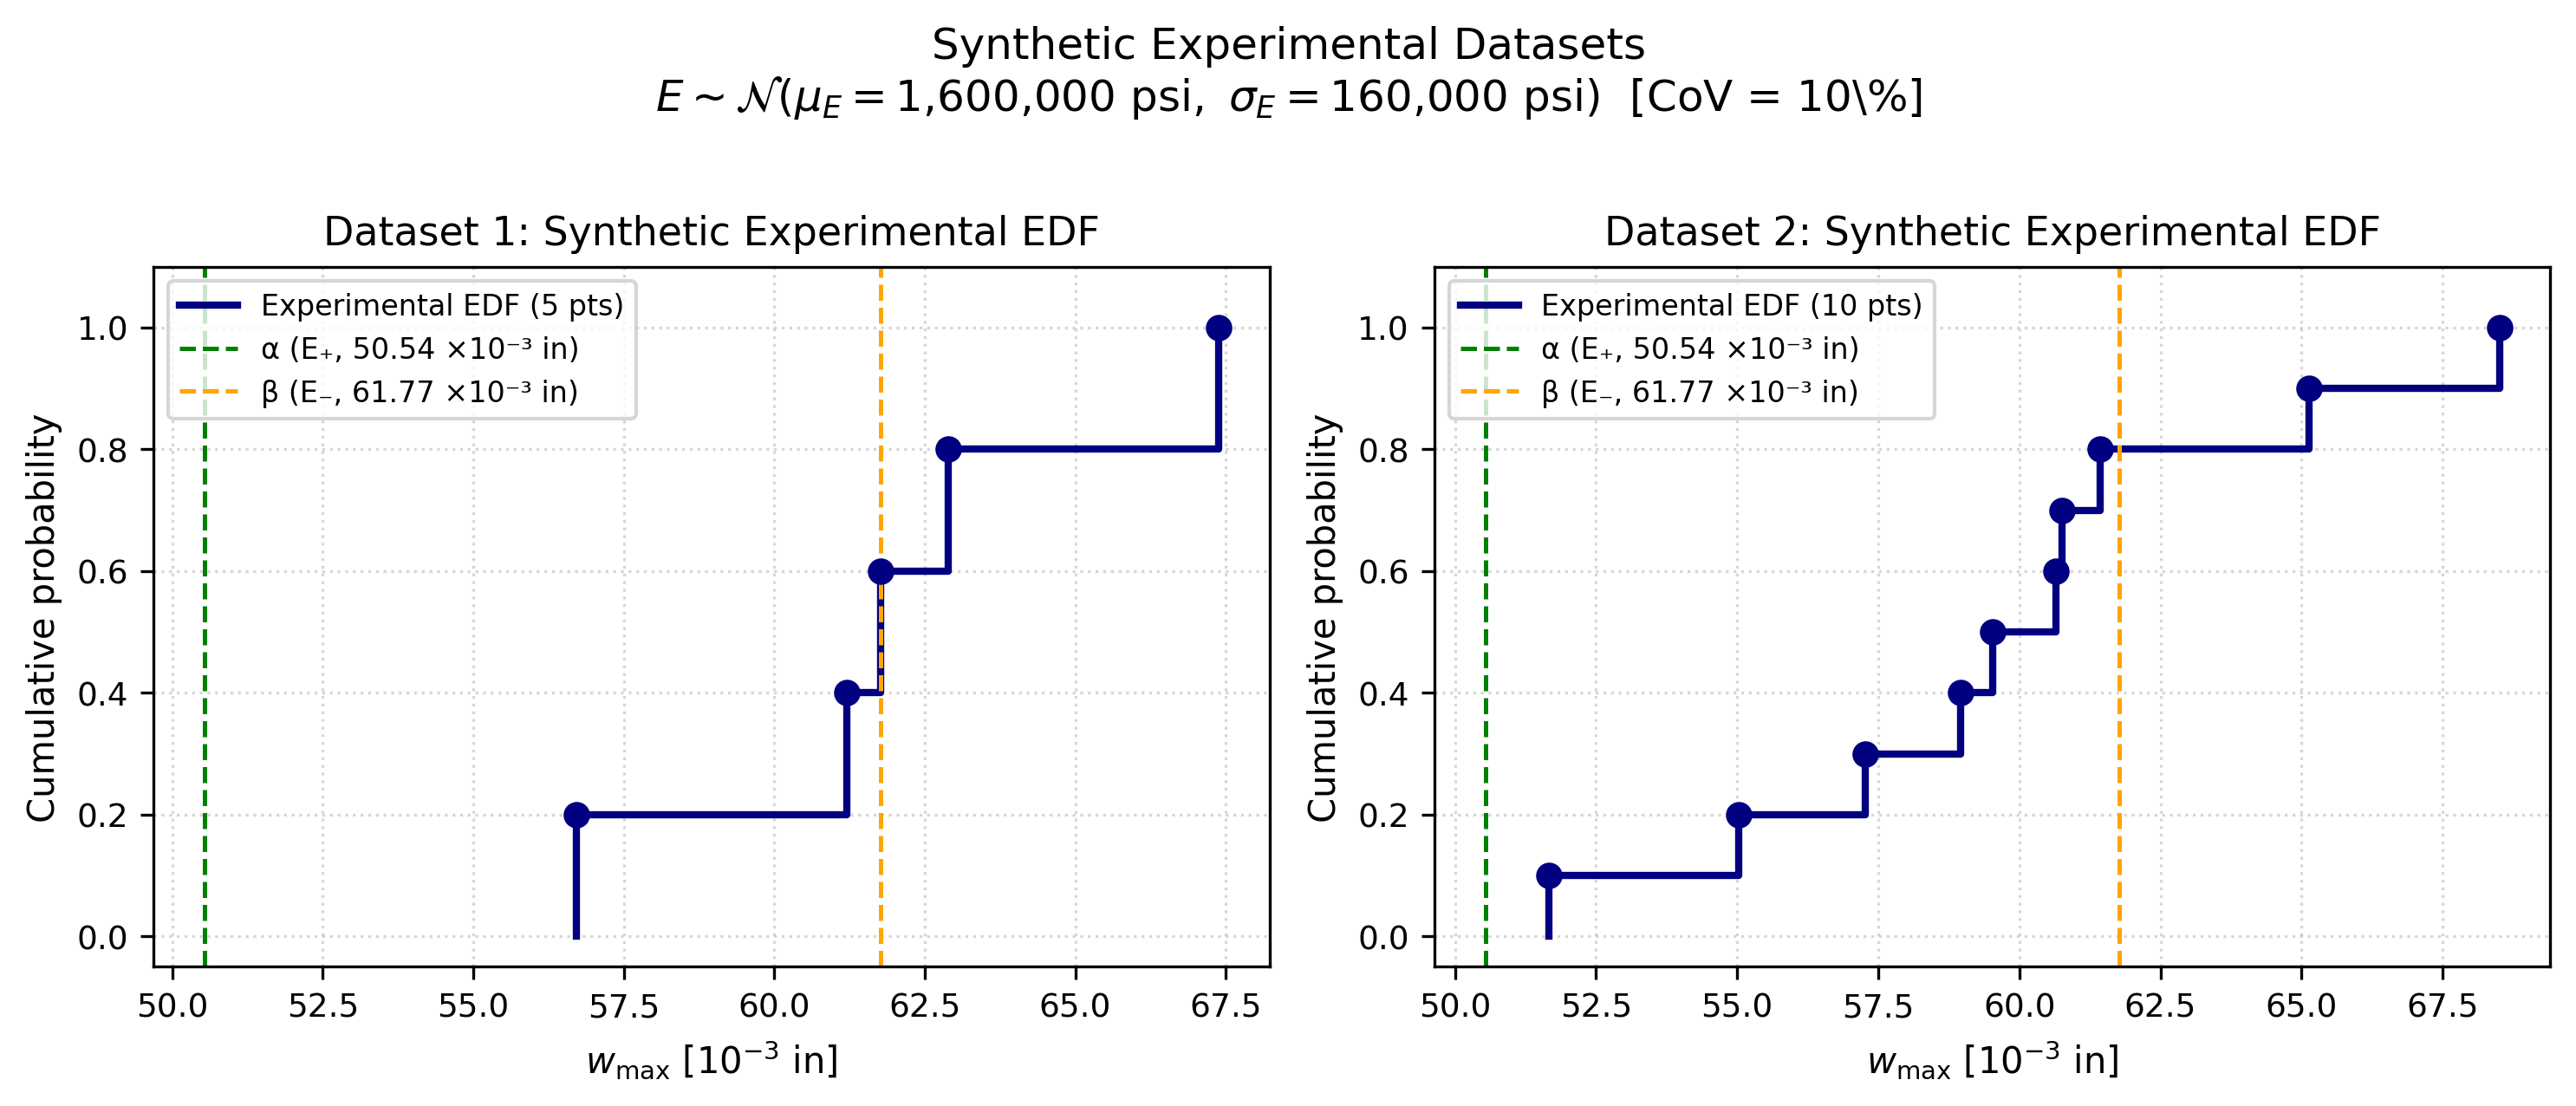
\includegraphics[width=\linewidth]{../hw5_figures/fig1_datasets.pdf}
  \caption{Synthetic experimental datasets (CDF) at $q_0=500$~lb/ft.
    Black dashed line: model prediction (nominal $E$).}
  \label{fig:hw5_data}
\end{figure}

\subsection{Area Validation Metric}
\label{sec:avm}

The Area Validation Metric (AVM) and its modified form (MAVM) of
Ferson~\textit{et al.}~\cite{ferson2008} are computed as:
\begin{equation}
  \mathrm{AVM} = \int\bigl|F_{\rm model}(y) - F_{\rm exp}(y)\bigr|\,dy,
  \label{eq:avm}
\end{equation}
with MAVM retaining sign information (positive when model under-predicts).
At $q_0=500$~lb/ft, Dataset~2, $n=100$:
$\mathrm{AVM}=2.139\times10^{-3}$~in,
$\mathrm{MAVM}=+1.079\times10^{-3}$~in.
The positive MAVM indicates the model slightly under-predicts deflection
at nominal conditions---a conservative bias for deflection-limited design.

\begin{figure}[ht]
  \centering
  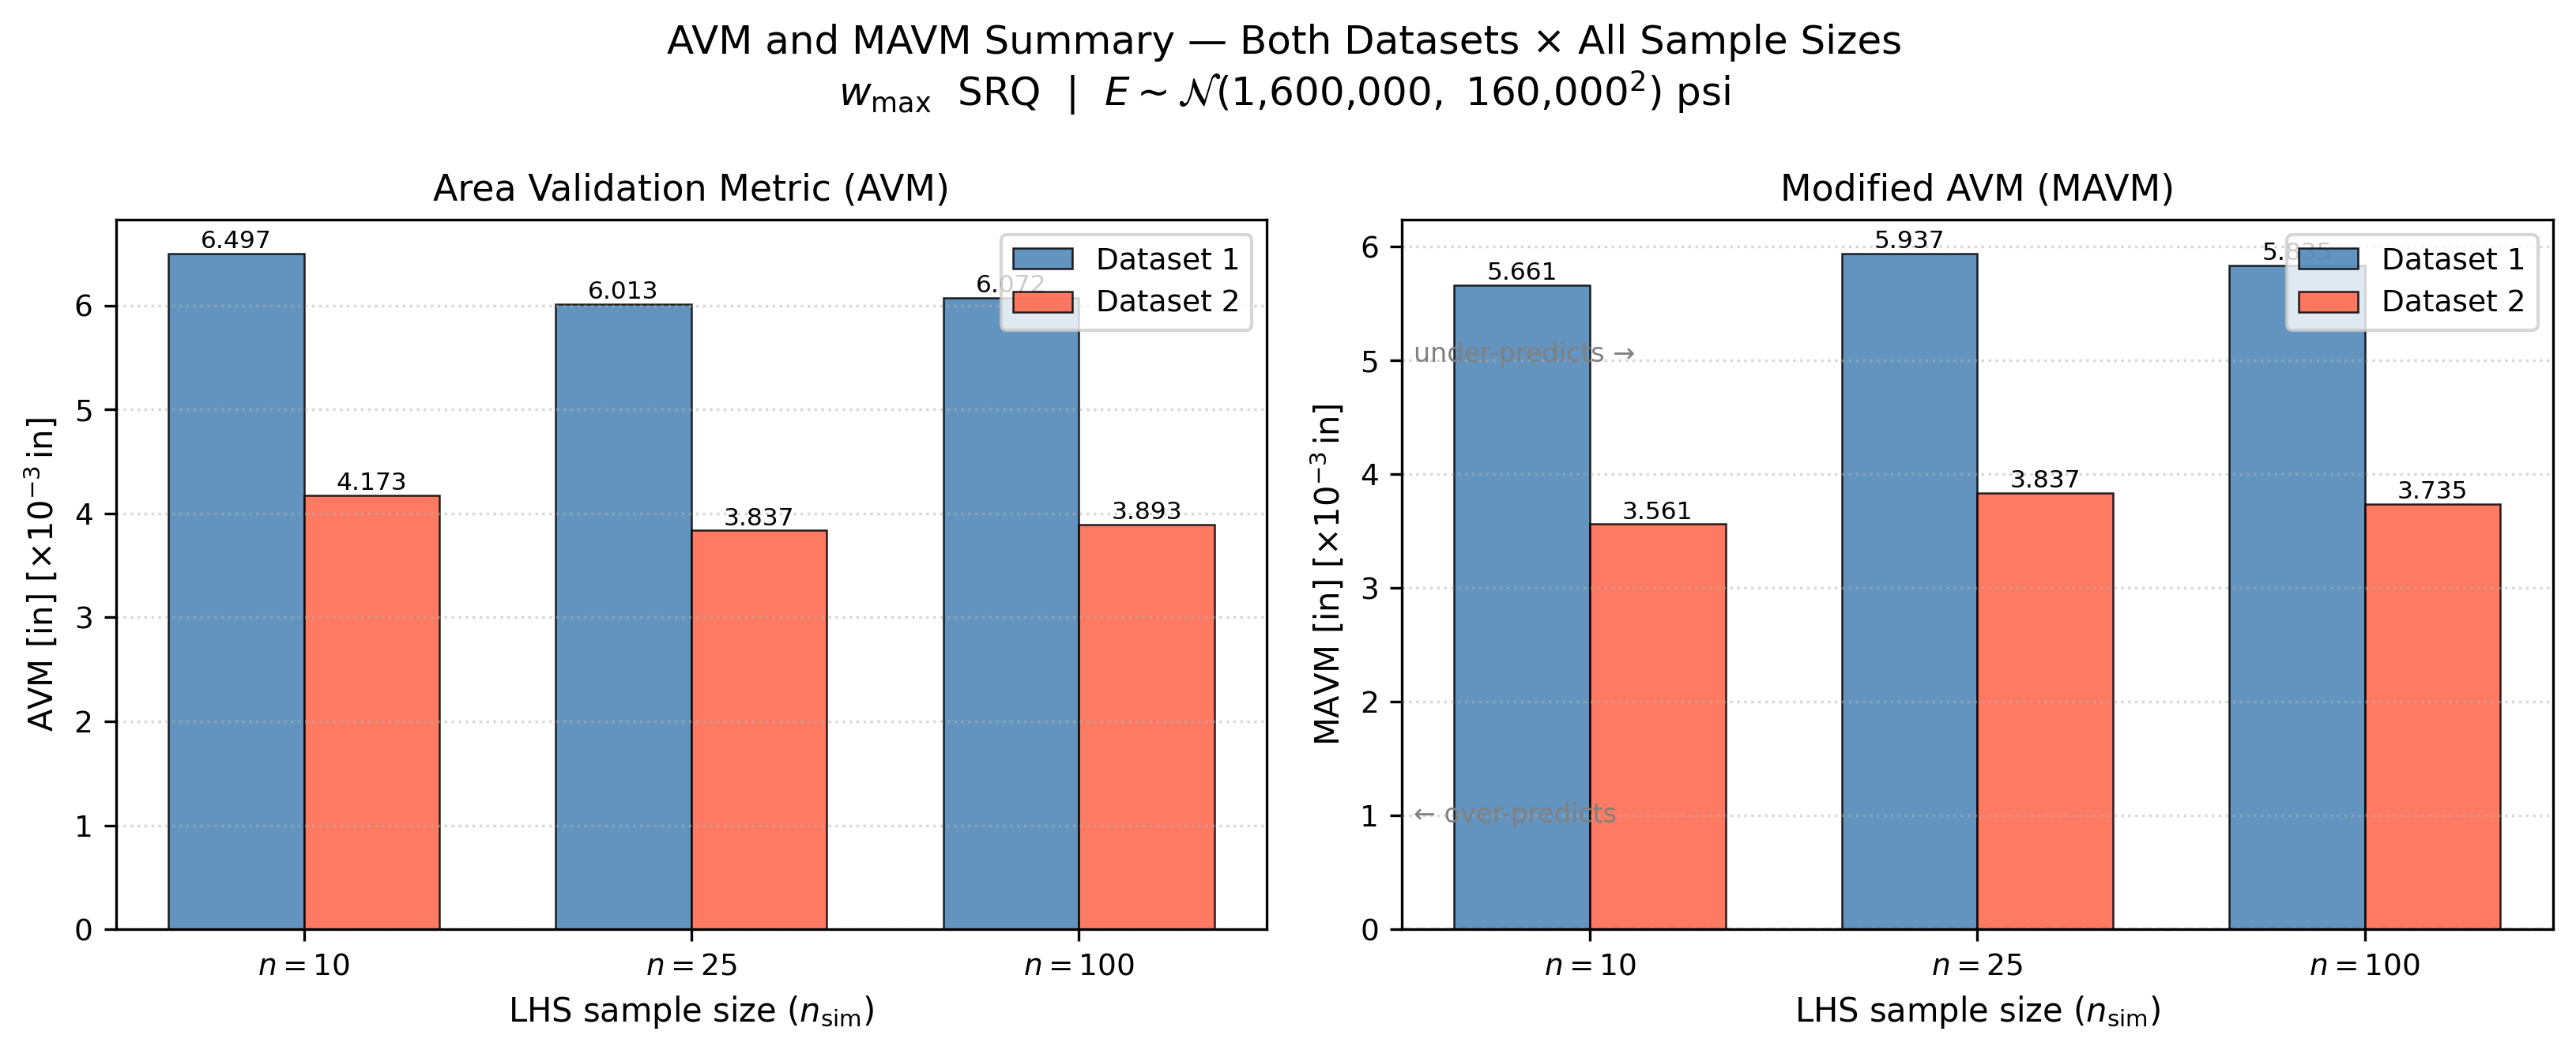
\includegraphics[width=\linewidth]{../hw5_figures/fig4_avm_mavm_bar.pdf}
  \caption{AVM and MAVM bar chart for varying dataset and sample size.
    MAVM $>0$ (conservative) at all conditions with $n\geq25$.}
  \label{fig:hw5_avm}
\end{figure}

%% ============================================================
\section{Predictive Uncertainty Quantification}
\label{sec:project}

\subsection{Uncertainty Sources and Treatment}
\label{sec:sources}

Two distinct uncertainty sources are propagated to $w_{\rm max}$:
\begin{itemize}[leftmargin=*, itemsep=0pt]
  \item \textbf{Aleatory (irreducible):}
    Elastic modulus $E\sim\mathcal{N}(1{,}600{,}000,\,160{,}000)$~psi
    (CoV~=~10\%), reflecting within-production variability of LVL.
  \item \textbf{Epistemic (reducible):}
    Uniformly distributed floor load $q_0\in[400,600]$~lb/ft
    ($\pm20\%$ of nominal), representing incomplete knowledge
    of occupancy loading.
\end{itemize}

Combining these two types under a single probabilistic model would
inappropriately collapse reducible uncertainty into the tails of the
predicted CDF.
Instead, we apply nested sampling to produce a p-box (probability box)
that explicitly separates the two types~\cite{roy2011, ferson2004}.

\subsection{Nested Sampling Methodology}
\label{sec:nested}

The outer loop partitions the epistemic interval $[q_{0,\rm lo},q_{0,\rm hi}]$
into $N_e$ equal sub-intervals, sampling $q_0$ at the $N_e+1$ partition
boundaries.
For each outer point, $N_a=100$ inner LHS samples of $E$ are drawn and
$w_{\rm max}$ evaluated at grid $N=20$.
This produces $N_e+1$ empirical CDFs whose pointwise minimum and maximum
define the p-box lower and upper envelopes:
\begin{align}
  F_{\rm lo}(y) &= \min_{j}\,\hat{F}_j(y),\\
  F_{\rm hi}(y) &= \max_{j}\,\hat{F}_j(y).
\end{align}

Convergence of the p-box with respect to $N_e$ is shown in
Figure~\ref{fig:pbox}.
The p-box stabilises by $N_e=10$; all four configurations
($N_e=5,10,25,100$) give consistent envelope bounds (Table~\ref{tab:pbox}).

\begin{figure*}[ht]
  \centering
  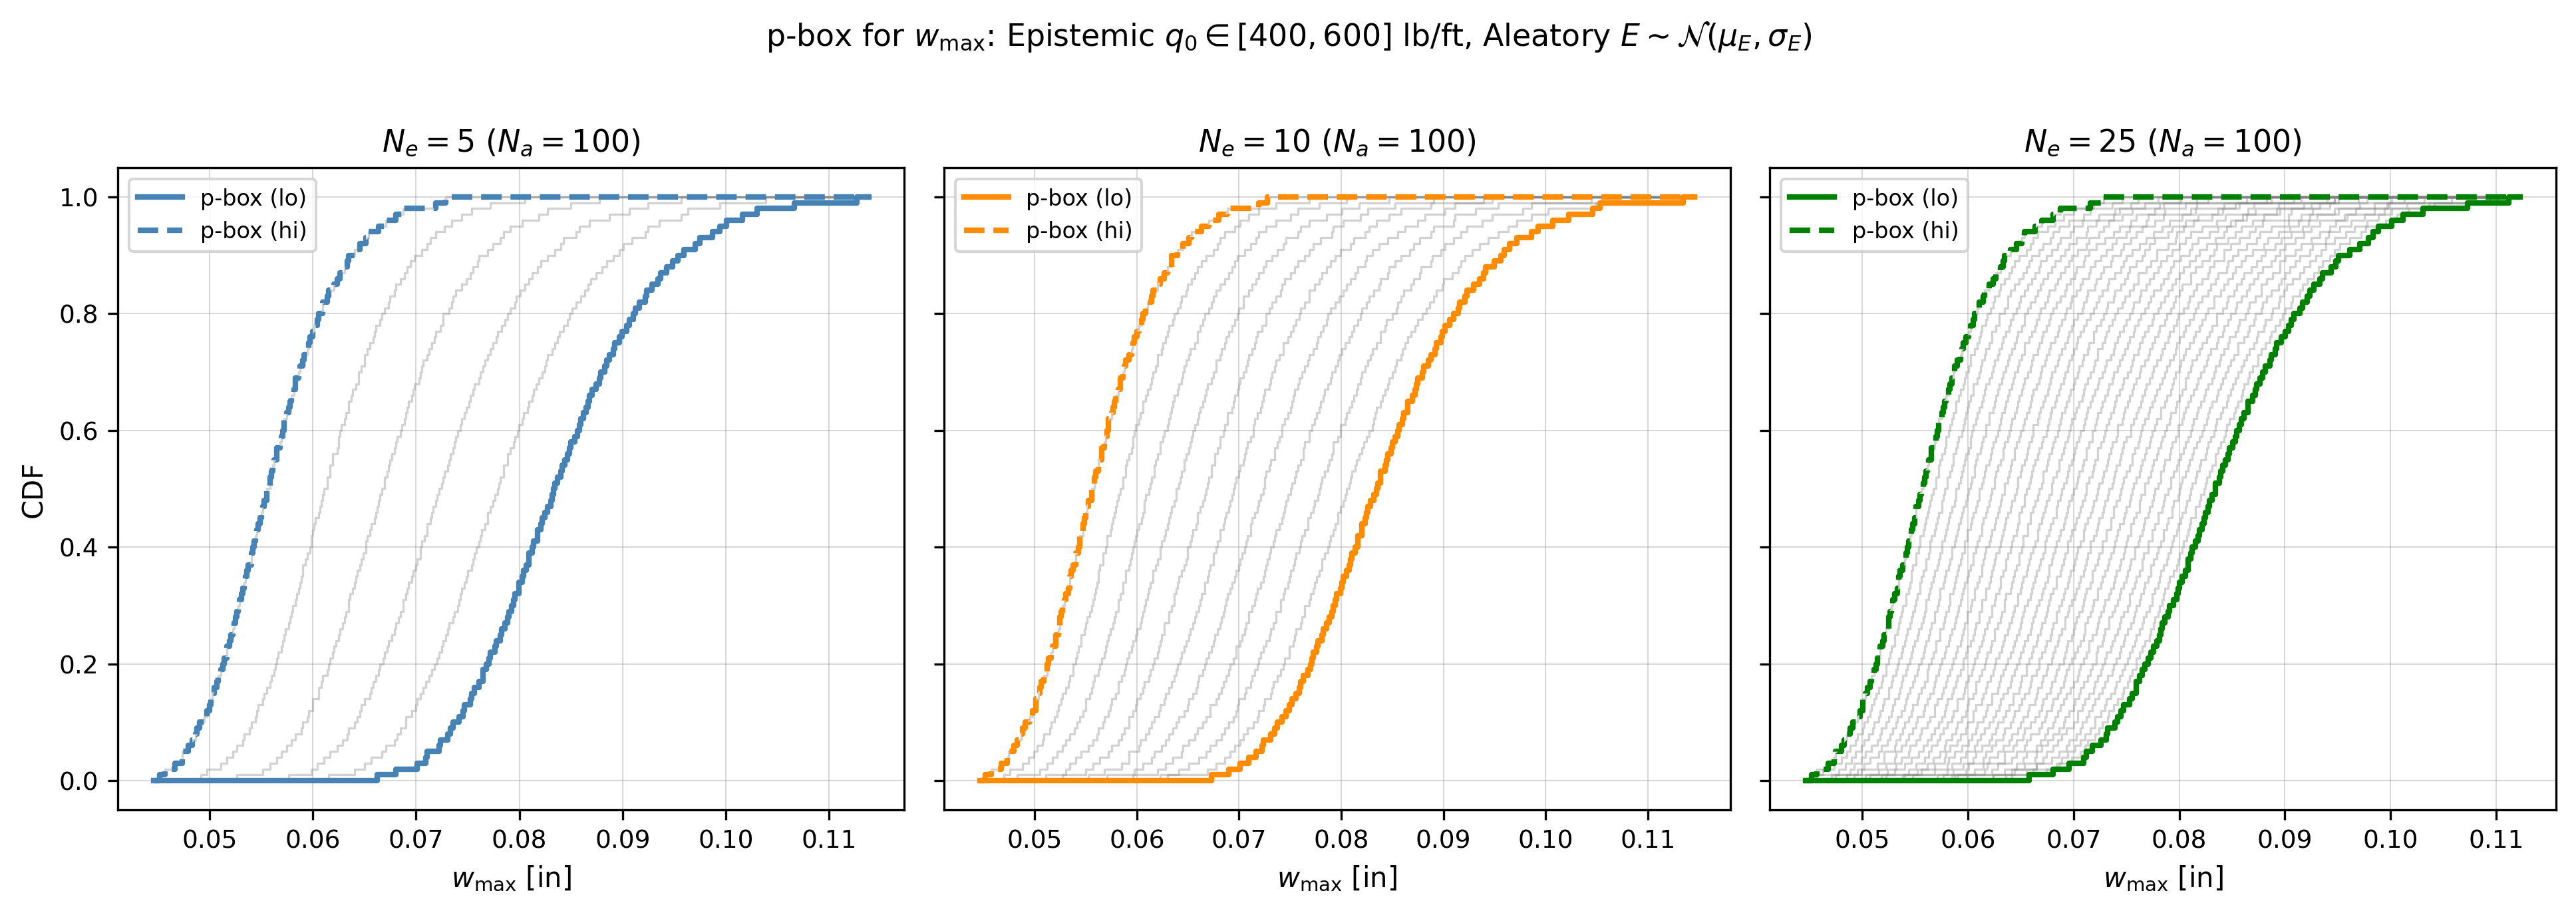
\includegraphics[width=\linewidth]{../project_figures/fig1_pbox.pdf}
  \caption{P-box for $w_{\rm max}$ using nested sampling.
    Gray lines: individual CDFs for each $q_0$ outer sample.
    Colored bounds: lower and upper p-box envelopes.
    From left to right: $N_e=5$, $10$, $25$, $100$.}
  \label{fig:pbox}
\end{figure*}

\begin{table}[ht]
\centering
\caption{P-box quantile intervals [lo, hi] (in) for $w_{\rm max}$.}
\label{tab:pbox}
\footnotesize
\setlength{\tabcolsep}{3pt}
\begin{tabular}{@{}rllll@{}}
\toprule
$N_e$ & \multicolumn{1}{c}{5th pct} & \multicolumn{1}{c}{50th pct} & \multicolumn{1}{c}{95th pct}\\
\midrule
  5 & [0.0474,\,0.0711] & [0.0556,\,0.0833] & [0.0664,\,0.0994]\\
 10 & [0.0474,\,0.0717] & [0.0556,\,0.0835] & [0.0664,\,0.0993]\\
 25 & [0.0475,\,0.0712] & [0.0556,\,0.0834] & [0.0663,\,0.0989]\\
100 & [0.0475,\,0.0714] & [0.0556,\,0.0833] & [0.0664,\,0.0997]\\
\bottomrule
\end{tabular}
\end{table}

\subsection{P-box vs.\ Uniform Epistemic Treatment}
\label{sec:comparison}

Figure~\ref{fig:pbox_uniform} compares the $N_e=25$ p-box with a
single CDF obtained by treating $q_0$ as uniformly distributed
$U[400,600]$~lb/ft (probabilistic epistemic treatment).
The uniform-CDF lies within the p-box but narrows the tails,
potentially under-reporting the probability of extreme deflections.
At the 95th percentile, the uniform single-CDF underestimates
the upper bound by $\approx0.012$~in (12\%), demonstrating that
collapsing epistemic uncertainty yields a non-conservative prediction.

\begin{figure}[ht]
  \centering
  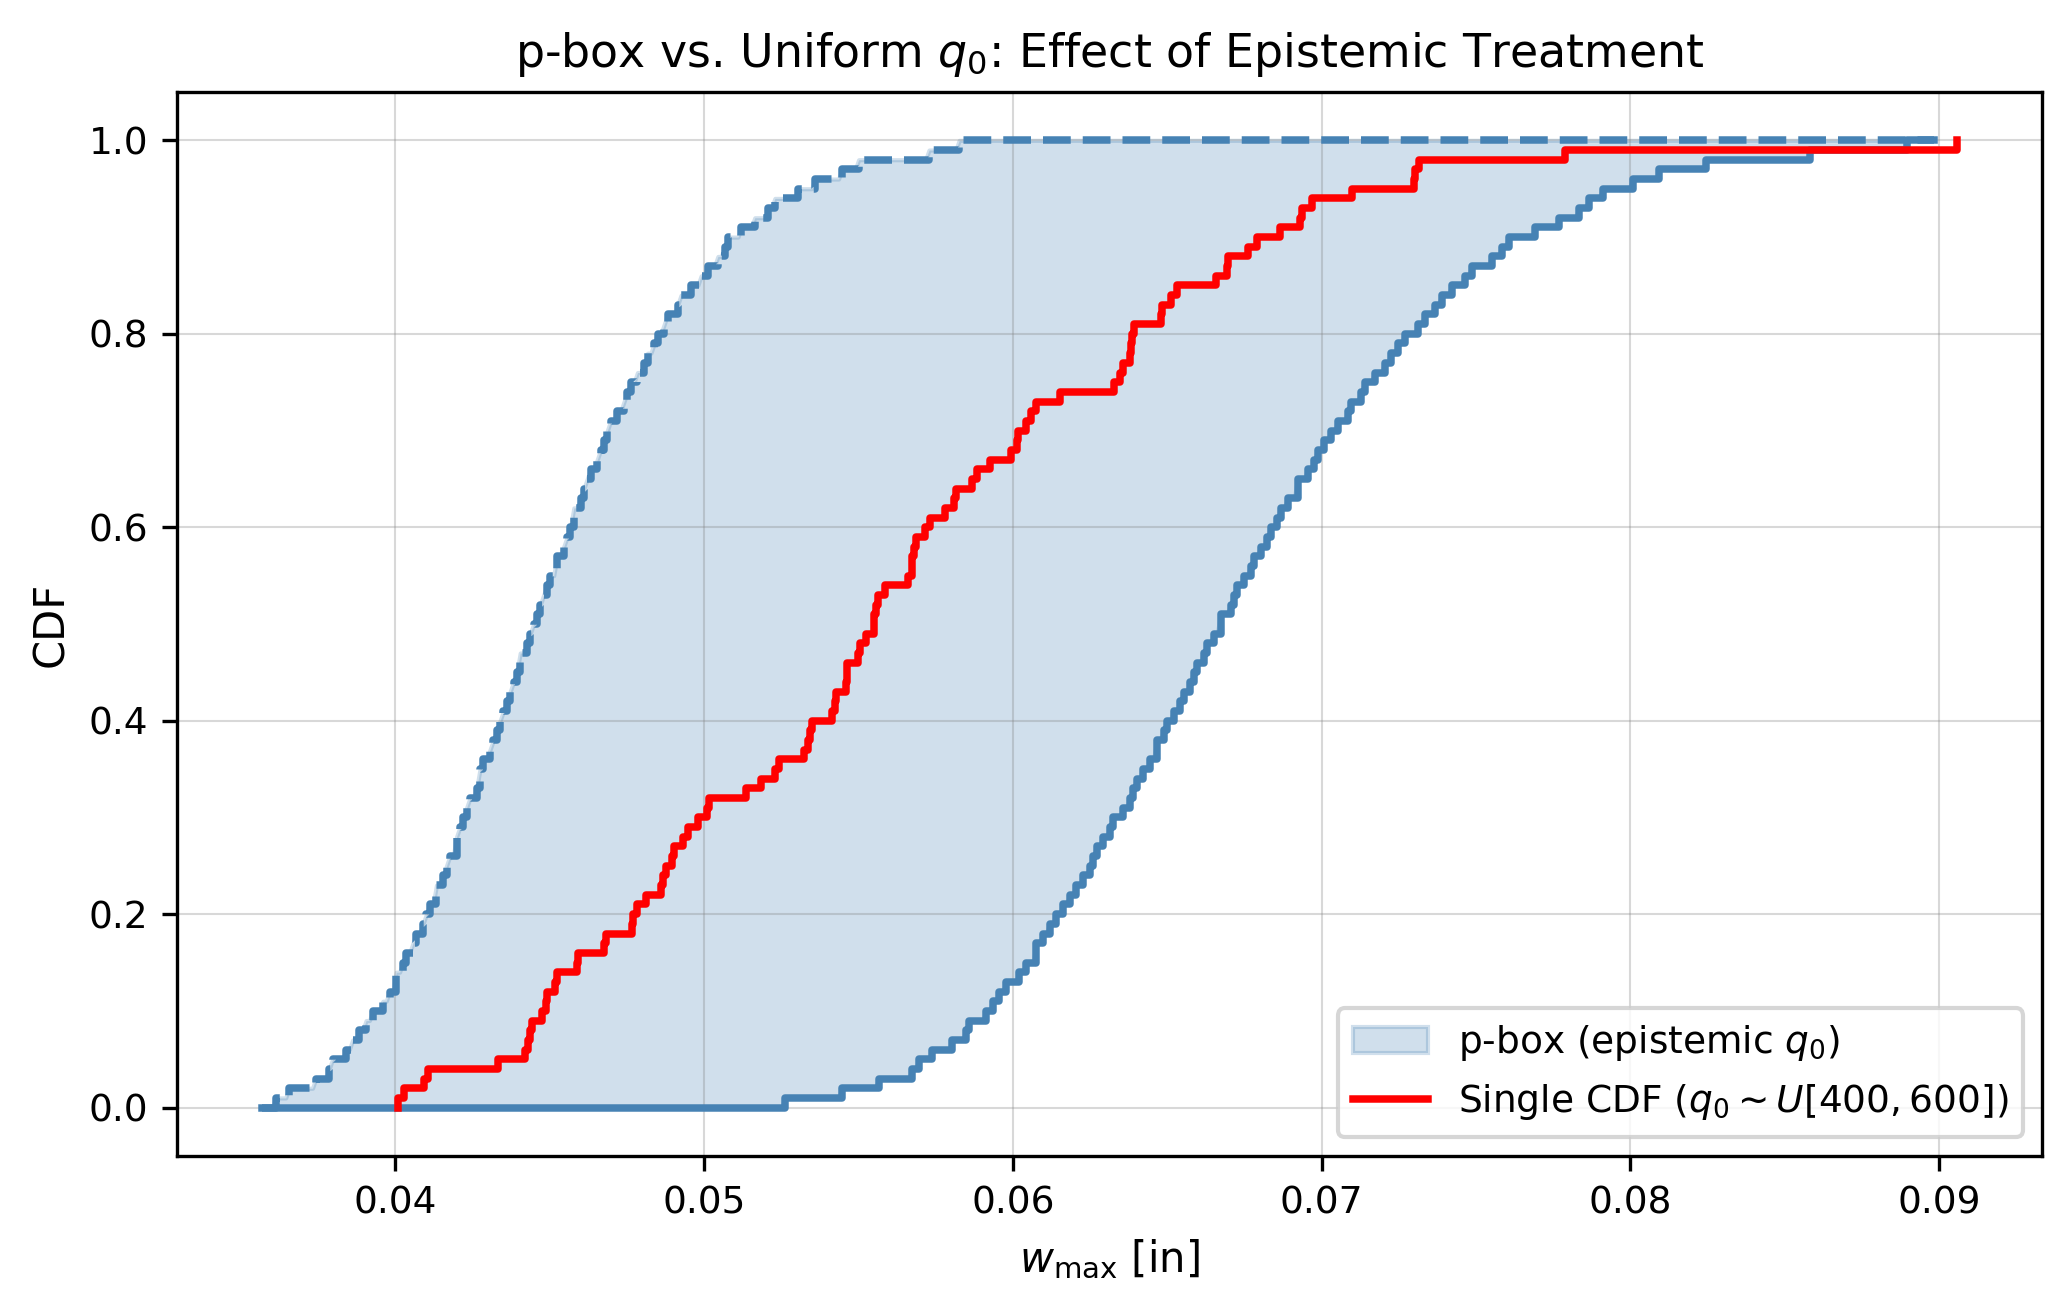
\includegraphics[width=\linewidth]{../project_figures/fig2_pbox_vs_uniform.pdf}
  \caption{P-box ($N_e=25$, blue band) vs.\ single CDF with
    $q_0\sim U[400,600]$~lb/ft (red).
    The uniform CDF collapses epistemic bounds, underestimating
    tail deflection.}
  \label{fig:pbox_uniform}
\end{figure}

\subsection{Model Form Uncertainty Extrapolation}
\label{sec:mf}

Validation was performed at $q_0=500$~lb/ft, but predictions are
sought up to $q_0=600$~lb/ft.
Because the Modified AVM (MAVM) was used as the validation metric,
the project requires separate extrapolation of its two components
(Roy \& Oberkampf~\cite{roy2011}):
\begin{align}
  d^+ &= \tfrac{1}{2}(\mathrm{AVM}+\mathrm{MAVM}) = 1.609\times10^{-3}~\text{in},\\
  d^- &= \tfrac{1}{2}(\mathrm{AVM}-\mathrm{MAVM}) = 0.530\times10^{-3}~\text{in}.
\end{align}
$d^+$ is the area where $F_{\rm sim}>F_{\rm exp}$ (model under-predicts);
$d^-$ is the area where $F_{\rm exp}>F_{\rm sim}$ (model over-predicts).
Five hypothetical validation points
at $q_0\in\{350,400,450,500,550\}$~lb/ft are assumed proportional to
deflection magnitude (linear in $q_0$), and separate linear regressions
are fitted (Figure~\ref{fig:mf_extrap}):
\begin{align}
  d^+(q_0) &= -4.37\times10^{-5} + 3.32\times10^{-6}\,q_0, \nonumber\\
           &\quad R^2=0.998, \\
  d^-(q_0) &= +1.34\times10^{-5} + 1.03\times10^{-6}\,q_0, \nonumber\\
           &\quad R^2=0.999.
\end{align}
At $q_0=600$~lb/ft, the upper 95\% prediction intervals give the
asymmetric model form interval:
\begin{align}
  U_{\rm MF}^+ &= 2.003\times10^{-3}~\text{in}\quad\text{(upper/right shift)},\\
  U_{\rm MF}^- &= 0.642\times10^{-3}~\text{in}\quad\text{(lower/left shift)}.
\end{align}

\begin{figure}[ht]
  \centering
  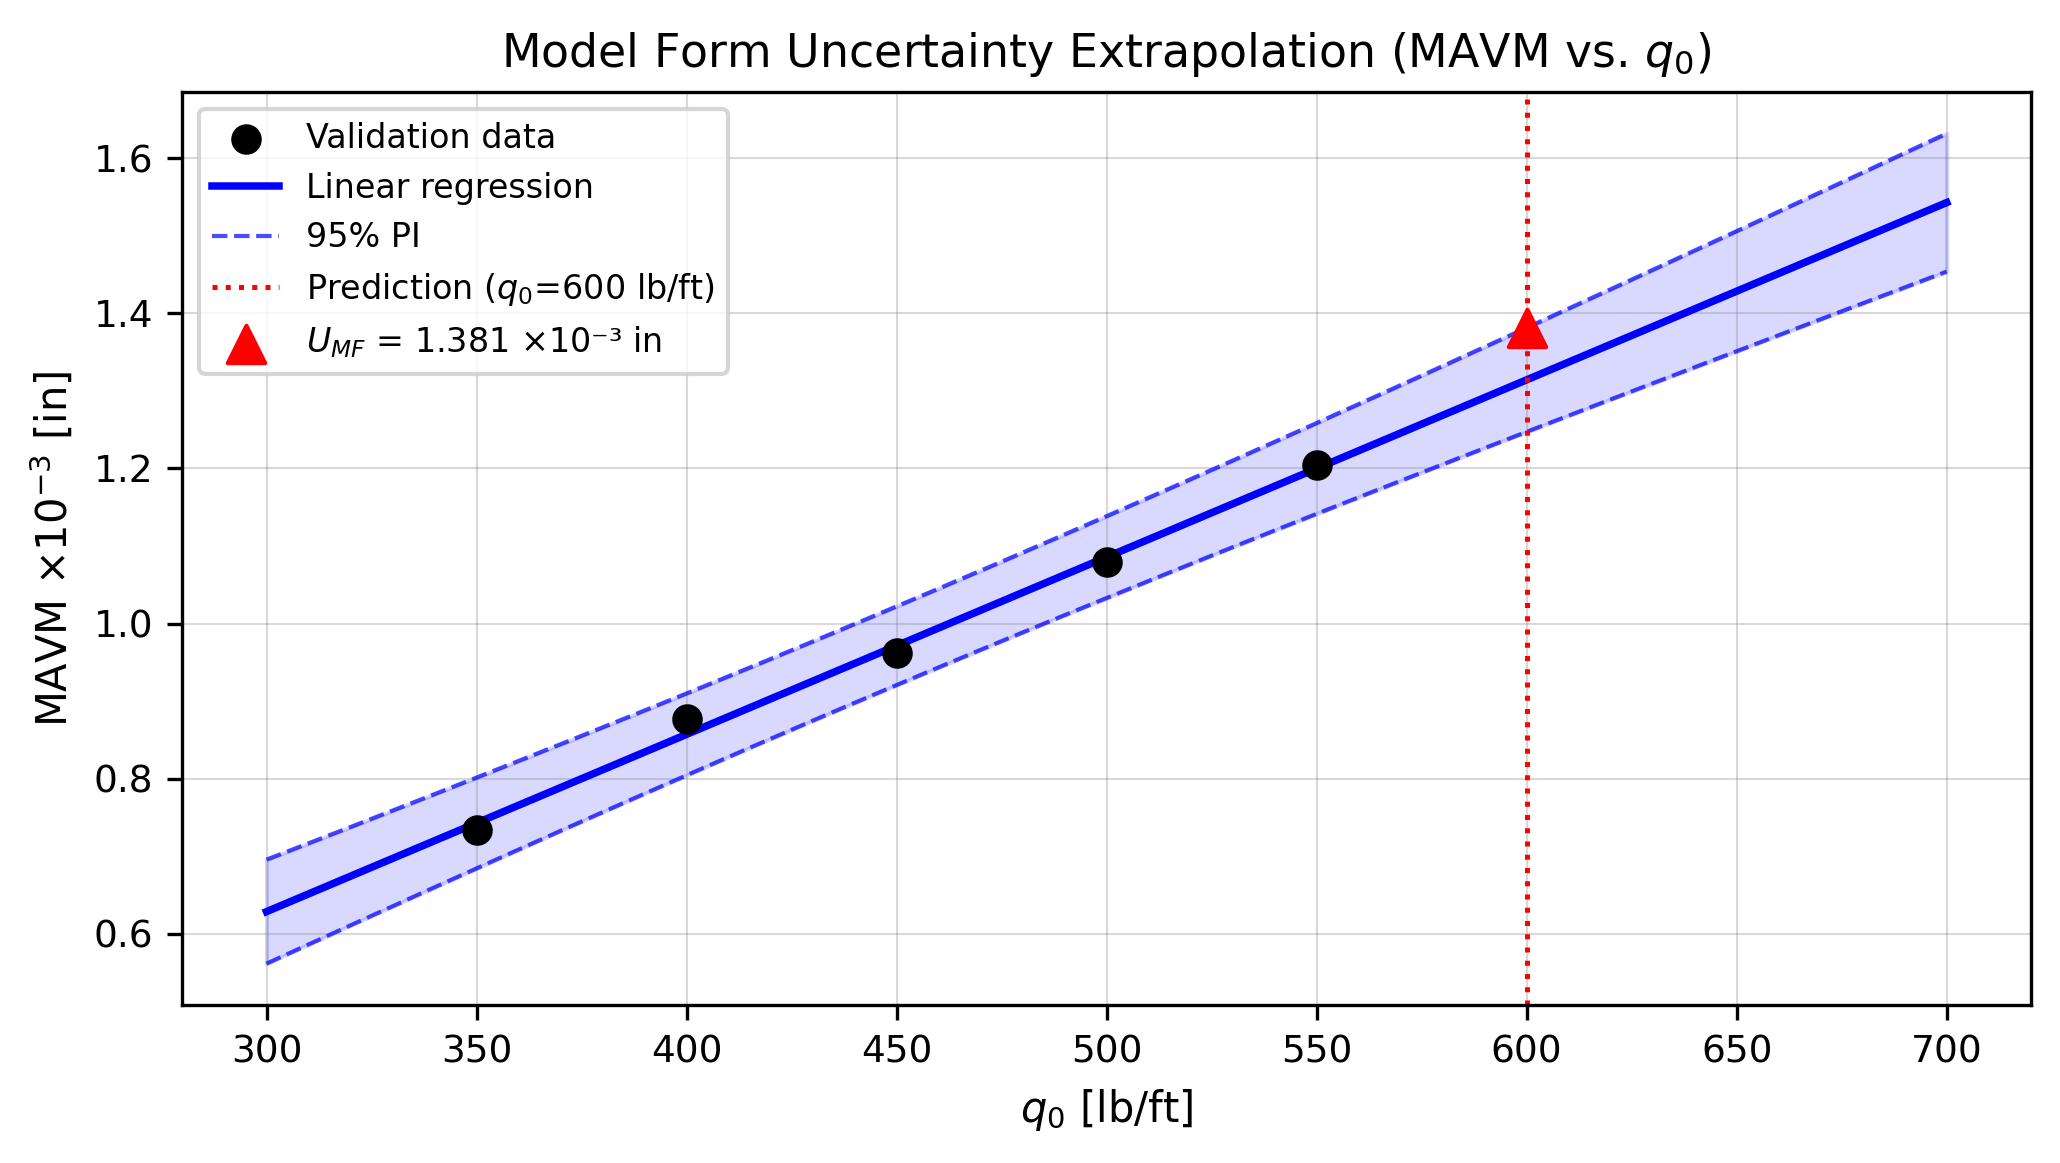
\includegraphics[width=\linewidth]{../project_figures/fig3_model_form_extrap.pdf}
  \caption{$d^+$ and $d^-$ vs.\ $q_0$ with separate linear regressions (solid),
    95\% prediction intervals (dashed/shaded), and extrapolated
    $U_{\rm MF}^+$, $U_{\rm MF}^-$ at $q_0=600$~lb/ft.
    Left: $d^+$ (model under-predicts region).  Right: $d^-$ (over-predicts region).}
  \label{fig:mf_extrap}
\end{figure}

\subsection{Total Predictive Uncertainty}
\label{sec:total}

The total uncertainty in $w_{\rm max}$ at $q_0=600$~lb/ft is
assembled additively per uncertainty source and side:
\begin{itemize}[leftmargin=*, itemsep=0pt]
  \item \textit{Input p-box}: inner-most band from nested sampling.
  \item \textit{Model form}: asymmetric expansion—shift upper envelope
    rightward by $U_{\rm MF}^+$; shift lower envelope leftward by $U_{\rm MF}^-$.
  \item \textit{Numerical}: symmetric further expansion by $U_{\rm NUM}^{\rm max}$.
\end{itemize}
Table~\ref{tab:budget} lists all components; Figure~\ref{fig:total}
shows the resulting layered CDF bands (matching the course reference figure).
Note that $U_{\rm NUM}^{\rm max}=2.60\times10^{-4}$~in ($0.31\%$ of $w_{\rm nom}$)
is physically too small to appear as a visible filled band at the plot scale; it is
rendered as crimson boundary lines with a bracket annotation at $F=0.50$ in
Figure~\ref{fig:total}.

\begin{table}[ht]
\centering
\caption{Total uncertainty budget at $q_0=600$~lb/ft,
  $w_{\rm nom}=0.0842$~in.}
\label{tab:budget}
\footnotesize
\setlength{\tabcolsep}{3pt}
\begin{tabular}{@{}p{2.8cm}rrp{0.9cm}@{}}
\toprule
Source & Mag.~[in] & \% $w_{\rm nom}$ & Side\\
\midrule
Aleatory ($E{\sim}\mathcal{N}$, 5--95\%) & 1.159e$-$2 & 13.77 & both\\
Epistemic ($q_0$ p-box) & 1.390e$-$2 & 16.52 & both\\
$U_{\rm MF}^+$ (95\% PI) & 2.003e$-$3 &  2.38 & upper\\
$U_{\rm MF}^-$ (95\% PI) & 6.42e$-$4  &  0.76 & lower\\
$U_{\rm NUM}^{\rm max}$ (corner) & 2.601e$-$4 &  0.31 & both\\
\midrule
\textbf{Total upper} & \textbf{2.776e$-$2} & \textbf{32.98} &\\
\textbf{Total lower} & \textbf{2.640e$-$2} & \textbf{31.36} &\\
\bottomrule
\end{tabular}
\end{table}

\begin{figure}[ht]
  \centering
  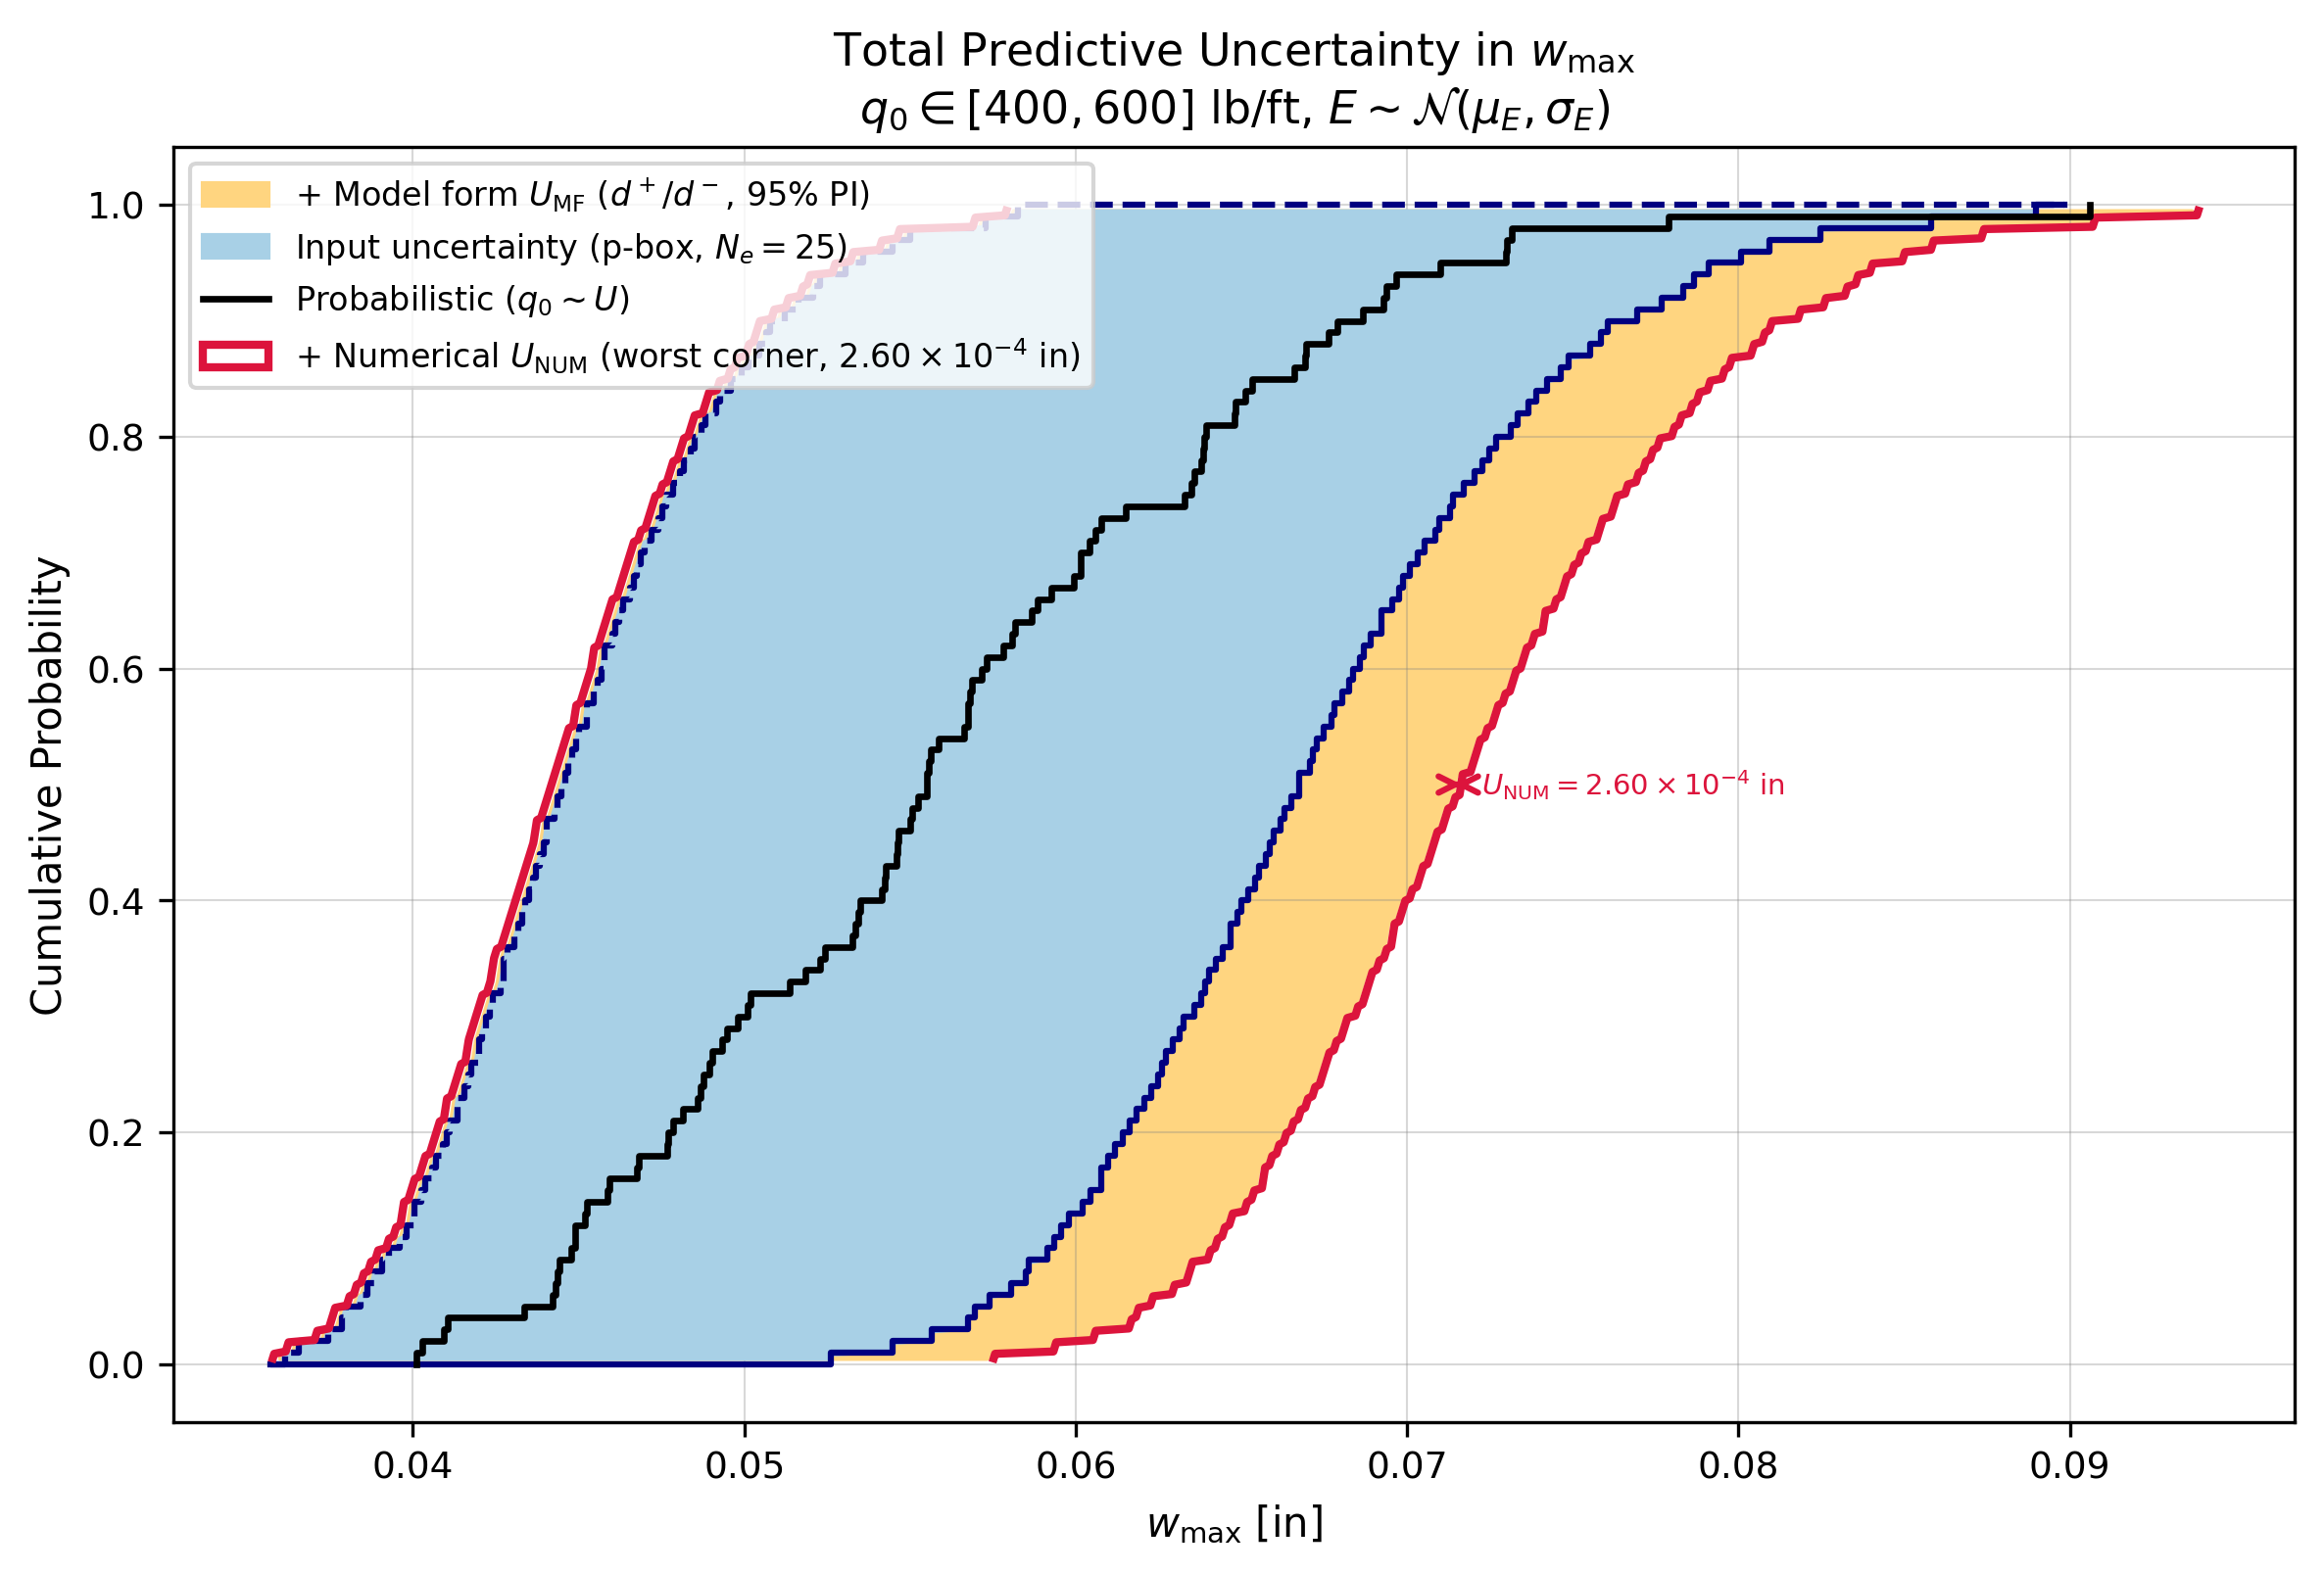
\includegraphics[width=\linewidth]{../project_figures/fig4_total_uncertainty.pdf}
  \caption{Total predictive uncertainty band in CDF space.
    Blue (innermost): input p-box ($N_e=25$);
    orange: asymmetric model form expansion ($U_{\rm MF}^+$ upper, $U_{\rm MF}^-$ lower);
    crimson lines (outermost): total envelope including $U_{\rm NUM}^{\rm max}=2.60\times10^{-4}$~in.
    Because $U_{\rm NUM}$ is only $0.31\%$ of $w_{\rm nom}$ it is physically too small
    to render as a visible filled band and is shown instead as boundary lines with a
    labeled bracket annotation at the 50th percentile.
    Black line: single CDF treating $q_0\sim U[400,600]$ probabilistically.}
  \label{fig:total}
\end{figure}

%% ============================================================
\section{Discussion}
\label{sec:discussion}

\subsection{Dominance Analysis}
\label{sec:dom}

The budget in Table~\ref{tab:budget} reveals a clear hierarchy:
\begin{enumerate}[leftmargin=*, itemsep=0pt]
  \item \emph{Epistemic load uncertainty} (17\%) is the largest
    single contributor, driven by the assumed $\pm20\%$ load range.
    Reducing it through site-specific load surveys would yield the
    greatest predictive improvement.
  \item \emph{Aleatory modulus variability} (14\%) reflects fundamental
    within-production scatter; it cannot be eliminated but can be
    partially constrained by certified LVL grading.
  \item \emph{Model form error} ($U_{\rm MF}^+\approx2.4\%$,
    $U_{\rm MF}^-\approx0.8\%$) is asymmetric---the model
    systematically under-predicts deflection ($d^+>d^-$,
    $\mathrm{MAVM}>0$)---indicating that the EB assumption
    (neglecting shear deformation) is adequate but slightly
    non-conservative for this $L/d=8.5$ slender member.
  \item \emph{Numerical error} ($U_{\rm NUM}^{\rm max}=0.31\%$,
    worst corner) confirms that the $N=20$ parametric grid is
    more than sufficient; further refinement is unnecessary.
\end{enumerate}

\subsection{Conservatism Assessment}
\label{sec:cons}

The positive MAVM throughout the validation study (model consistently
under-predicts deflection) indicates that using the FD model for
deflection-limit-state design produces a conservative (safe-side) prediction.
Combined with the epistemic upper-bound treatment, the upper p-box
envelope at $q_0=600$~lb/ft, $w_{\rm max}^{\rm hi,95} = 0.099$~in,
provides a defensible design deflection that accounts for all
identified uncertainty sources.

For comparison, the allowable deflection per IBC~\cite{ibc2021} for
floor members is $L/360 = 0.267$~in for live loads, well above the
predicted upper bound.
This suggests the 8-ft LVL header is adequate with significant reserve
capacity even under the most adverse scenario explored here.

%% ============================================================
\section{Conclusions}
\label{sec:conc}

A structured VV\&UQ study of an Euler--Bernoulli finite-difference
beam solver for residential LVL header design leads to the following
conclusions:

\begin{enumerate}[leftmargin=*, itemsep=2pt]
  \item The FD code achieves the theoretical $\mathcal{O}(h^2)$
    convergence order ($p_{\rm obs}=2.000$) for all SRQs, confirming
    correct implementation.
  \item Numerical uncertainty at the parametric grid ($N=20$) is
    $U_{\rm NUM}=1.962\times10^{-4}$~in (0.28\%), negligible relative
    to physical input uncertainty.
  \item Model validation confirms a small, conservative (positive) MAVM
    across all dataset sizes, establishing the EB model as suitable
    for deflection-based design at the validation conditions.
  \item The p-box analysis reveals that treating epistemic load uncertainty
    probabilistically (uniform $q_0$) underestimates the 95th percentile
    deflection by approximately 12\% compared to the proper p-box treatment.
  \item Total predictive uncertainty spans 31--33\% of the nominal deflection
    at $q_0=600$~lb/ft (asymmetric: upper side 33\%, lower side 31\%
    due to the $d^+>d^-$ model bias).
    Epistemic load uncertainty and aleatory modulus variability together
    account for 30 of those 32 percentage points.
    Reducing load specification uncertainty is the highest-leverage
    improvement available.
  \item Despite all uncertainties, the predicted upper 95th percentile
    deflection ($0.099$~in) is well below the IBC allowable of $0.267$~in,
    confirming structural adequacy of the 8-ft LVL header.
\end{enumerate}

%% ============================================================
\section*{Acknowledgments}

The authors gratefully acknowledge Professor Christopher Roy for
guidance on the VV\&UQ methodology and for providing the course
framework that structured this study.

%% ============================================================
\bibliographystyle{aiaa}
\begin{thebibliography}{9}

\bibitem{asme2009}
ASME,
\textit{Standard for Verification and Validation in Computational Fluid
  Dynamics and Heat Transfer}, ASME V\&V~20, 2009.

\bibitem{roy2011}
C.~J.~Roy and W.~L.~Oberkampf,
``A comprehensive framework for verification, validation, and uncertainty
  quantification in scientific computing,''
\textit{Computer Methods in Applied Mechanics and Engineering},
Vol.~200, 2011, pp.~2131--2144.

\bibitem{roache1994}
P.~J.~Roache,
``Perspective: A method for uniform reporting of grid refinement studies,''
\textit{ASME Journal of Fluids Engineering},
Vol.~116, 1994, pp.~405--413.

\bibitem{celik2008}
I.~B.~Celik, U.~Ghia, P.~J.~Roache, C.~J.~Freitas, H.~Coleman, and P.~E.~Raad,
``Procedure for estimation and reporting of uncertainty due to discretization
  in CFD applications,''
\textit{ASME Journal of Fluids Engineering}, Vol.~130, 2008, 078001.

\bibitem{ferson2008}
S.~Ferson, W.~L.~Oberkampf, and L.~Ginzburg,
``Model validation and predictive capability for the thermal challenge problem,''
\textit{Computer Methods in Applied Mechanics and Engineering},
Vol.~197, 2008, pp.~2408--2430.

\bibitem{ferson2004}
S.~Ferson and W.~T.~Tucker,
``Sensitivity analysis using probability bounding,''
\textit{Reliability Engineering \& System Safety},
Vol.~91, 2006, pp.~1435--1442.

\bibitem{nds2018}
American Wood Council,
\textit{National Design Specification (NDS) for Wood Construction},
2018 Edition.

\bibitem{ibc2021}
International Code Council,
\textit{International Building Code}, 2021 Edition.

\end{thebibliography}

\end{document}
